\documentclass[tikz,border=6pt]{standalone}
\usepackage{xcolor}
\usetikzlibrary{arrows.meta}

\definecolor{shipblue}{HTML}{4A90D9}
\definecolor{linegray}{HTML}{333333}

\begin{document}
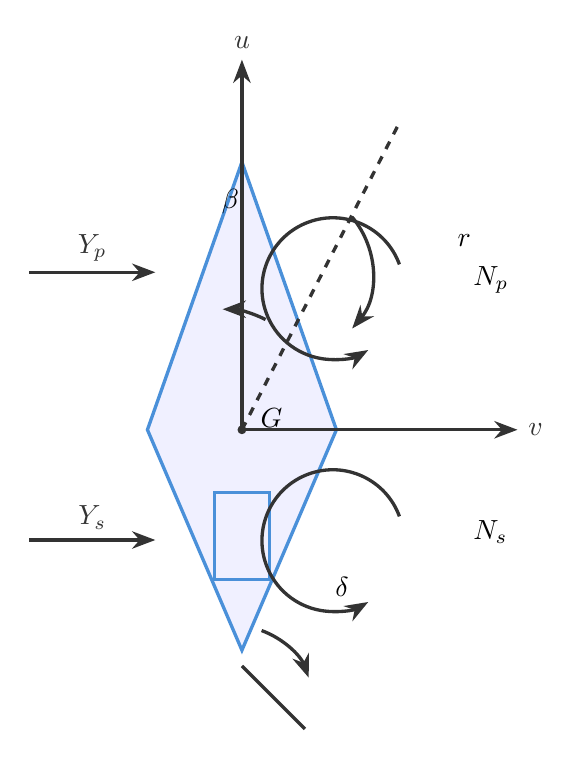
\begin{tikzpicture}[>=Stealth, line width=1.2pt]
  % ship body
  \draw[draw=shipblue, fill=blue!6] (0,0) -- (1.2,2.8) -- (0,6.2) -- (-1.2,2.8) -- cycle;
  \draw[draw=shipblue] (-0.35,0.9) rectangle (0.35,2.0);
  \fill[linegray] (0,2.8) circle (1.6pt);
  \node[right] at (0.1,2.95) {$G$};

  % axes and motions
  \draw[->, linegray] (0,2.8) -- (0,7.5) node[above] {$u$};
  \draw[->, linegray] (0,2.8) -- (3.5,2.8) node[right] {$v$};
  \draw[->, linegray] (1.4,5.5) arc[start angle=40,end angle=-40,radius=1.1cm];
  \node[right] at (2.6,5.2) {$r$};

  % rudder and drift
  \draw[linegray] (0,-0.2) -- (0.8,-1.0);
  \draw[->, linegray] (0.25,0.25) arc[start angle=70,end angle=20,radius=1.0cm];
  \node[right] at (1.05,0.8) {$\delta$};
  \draw[dashed, linegray] (0,2.8) -- (2.0,6.7);
  \draw[->, linegray] (0.3,4.2) arc[start angle=63,end angle=90,radius=1.2cm];
  \node[left] at (0.1,5.7) {$\beta$};

  % forces and moments
  \draw[->, linegray] (-2.7,4.8) -- (-1.1,4.8) node[midway, above] {$Y_p$};
  \draw[->, linegray] (-2.7,1.4) -- (-1.1,1.4) node[midway, above] {$Y_s$};
  \draw[->, linegray] (2.0,4.9) arc[start angle=20,end angle=300,radius=0.9cm];
  \node[right] at (2.8,4.7) {$N_p$};
  \draw[->, linegray] (2.0,1.7) arc[start angle=20,end angle=300,radius=0.9cm];
  \node[right] at (2.8,1.5) {$N_s$};
\end{tikzpicture}
\end{document}
